%!TEX root = ../main.tex
\begin{figure*}
	\plaatje{Roteer onze rendering zodat hij klopt met de blauwe rendering}
	\plaatje{In caption mention: material properties, light properties, tessellation levels.}
	\centering
	\begin{subfigure}[b]{0.2\textwidth}
		\centering
		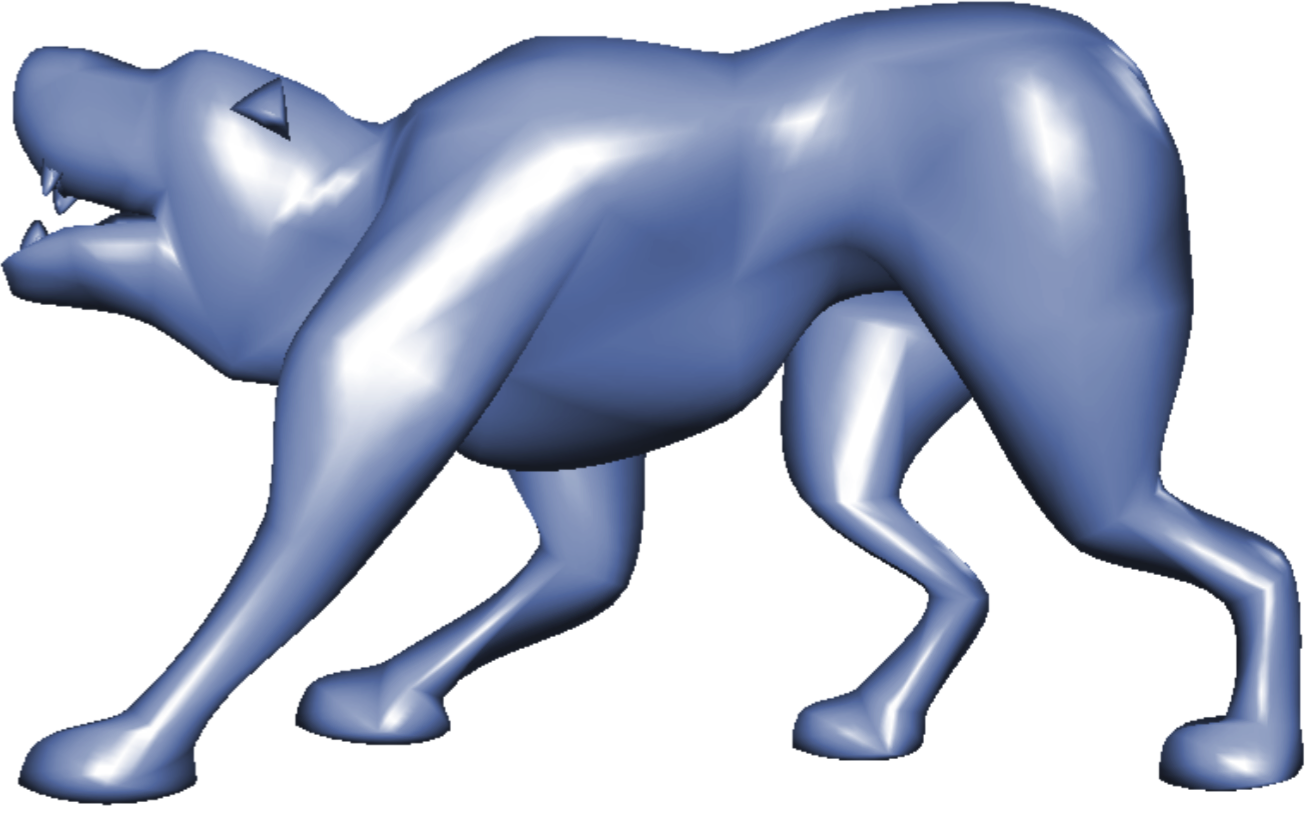
\includegraphics[width=\textwidth]{content/img/results/dogCPU.png}
		\caption{Rottweiler on CPU}
		\label{fig:results:cpugpu:cpuDog}
	\end{subfigure}
	\hspace{0.1\textwidth}
	\begin{subfigure}[b]{0.2\textwidth}
		\centering
		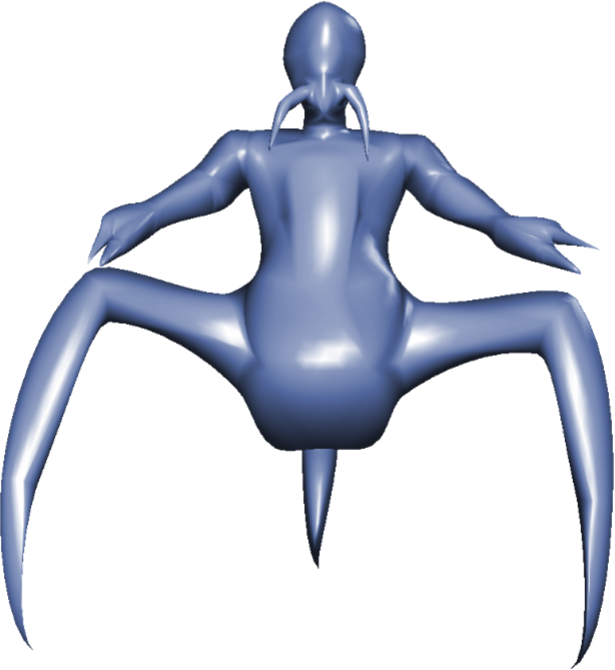
\includegraphics[width=\textwidth]{content/img/results/voreCPU.png}
		\caption{Vore on CPU}
		\label{fig:results:cpugpu:cpuVore}
	\end{subfigure}	
	\hspace{0.1\textwidth}
	\begin{subfigure}[b]{0.2\textwidth}
		\centering
		\includegraphics[width=\textwidth]{content/img/results/shamblercpu.png}
		\caption{Shambler on CPU}
		\label{fig:results:cpugpu:cpuShambler}
	\end{subfigure}		

	\begin{subfigure}[b]{0.2\textwidth}
		\centering
		\includegraphics[width=\textwidth]{content/img/results/doggpu.png}
		\caption{Rottweiler on GPU}
		\label{fig:results:cpugpu:gpuDog}
	\end{subfigure}
	\hspace{0.1\textwidth}
	\begin{subfigure}[b]{0.2\textwidth}
		\centering
		\includegraphics[width=\textwidth]{content/img/results/voregpu.png}
		\caption{Vore on GPU}
		\label{fig:results:cpugpu:gpuVore}
	\end{subfigure}	
	\hspace{0.1\textwidth}
	\begin{subfigure}[b]{0.2\textwidth}
		\centering
		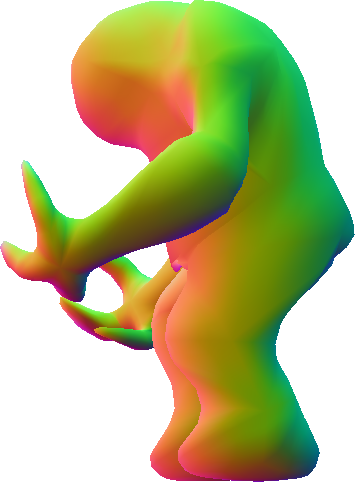
\includegraphics[width=\textwidth]{content/img/results/shamblerGPU.png}
		\caption{Shambler on GPU}
		\label{fig:results:cpugpu:gpuShambler}
	\end{subfigure}			
	\caption{A family of game characters from the game Quake 1. \subref{fig:results:cpugpu:cpuDog}, \subref{fig:results:cpugpu:cpuVore} and \subref{fig:results:cpugpu:cpuShambler} are rendered on a CPU by \citeauthor{vlachos2001curved}. \subref{fig:results:cpugpu:gpuDog}, \subref{fig:results:cpugpu:gpuVore}, \subref{fig:results:cpugpu:gpuShambler} are rendered by our implementation. Figures \subref{fig:results:cpugpu:cpuDog}, \subref{fig:results:cpugpu:cpuVore} and \subref{fig:results:cpugpu:cpuShambler} were taken from \textcite{vlachos2001curved}.}
	\label{fig:results:cpugpu}
\end{figure*}